% A generic network with internal coupling coefficients, external coupling and external stimulation.
% Author: Paula Sanz Leon
% Project: The Virtual Brain
% All contributed model should have an illustration with the main parameters on it

\documentclass{article}

\usepackage{tikz}
\usetikzlibrary{arrows}

\usepackage[margin=0in, paperwidth=3in, paperheight=2.2in]{geometry}

\definecolor{lavander}{cmyk}{0.58,0.48,0,0}
\def\lav{lavander!60}

\begin{document}
\pagestyle{empty}

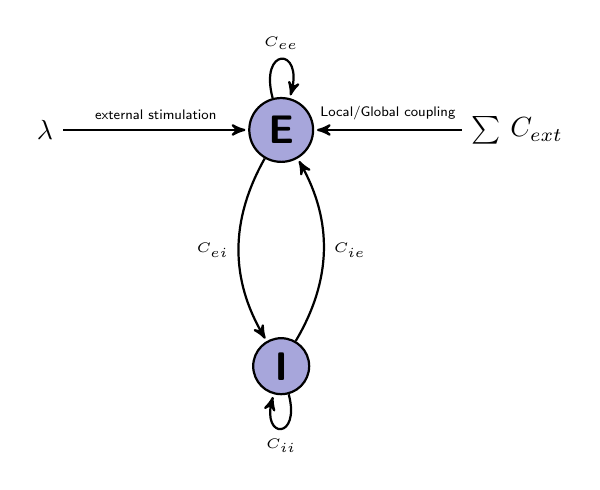
\begin{tikzpicture}[->,>=stealth',shorten >=1pt,auto,node distance=3cm,
  thick,main node/.style={circle,fill=\lav ,draw,font=\sffamily\Large\bfseries}]
  \begin{scope}
  	\node[main node] (1) {E};
  	\node[main node] (2) [below of=1] {I};
    \node (3) [left of=1]{$\lambda$};
    \node (4) [right of=1] {$\sum\,C_{ext}$};
    
  	\path[every node/.style={font=\sffamily\tiny}]
    	(1) edge [bend right] node[left] {$C_{ei}$} (2)
        	edge [loop above] node {$C_{ee}$} (1)
        	
    	(2) edge [bend right] node[right] {$C_{ie}$} (1)
        	edge [loop below] node {$C_{ii}$} (2)
        	
        (3) edge [right] node[above] {external stimulation} (1)
        (4) edge [right] node[above] {Local/Global coupling} (1);

        
   \end{scope}

\end{tikzpicture}

\end{document}